
\begin{frame}{Pourquoi un langage de programmation\,?}

SQL \alert{n'est pas} un langage de programmation
\begin{redbullet}

  \item SQL est un langage pensé pour permettre l'interrogation 
     d'une base de manière \alert{déclarative}, et non procédurale 
  
  \item Pas de variable, pas de boucle, pas de test
 
\end{redbullet}

\vfill

Pour écrire des applications, on utilise SQL associé à  un langage de programmation

\vfill
L'association\,:

\begin{redbullet}
  
  \item SQL pour les accès à la base
  \item Python, Java, PHP, C++, etc.  pour tout le reste

\end{redbullet}

\end{frame}

\begin{frame}{Deux architectures possibles}

Premier cas (à gauche)\,: les requêtes SQL sont intégrées à 
un \alert{programme client} et transmises au serveur de données.

\vfill

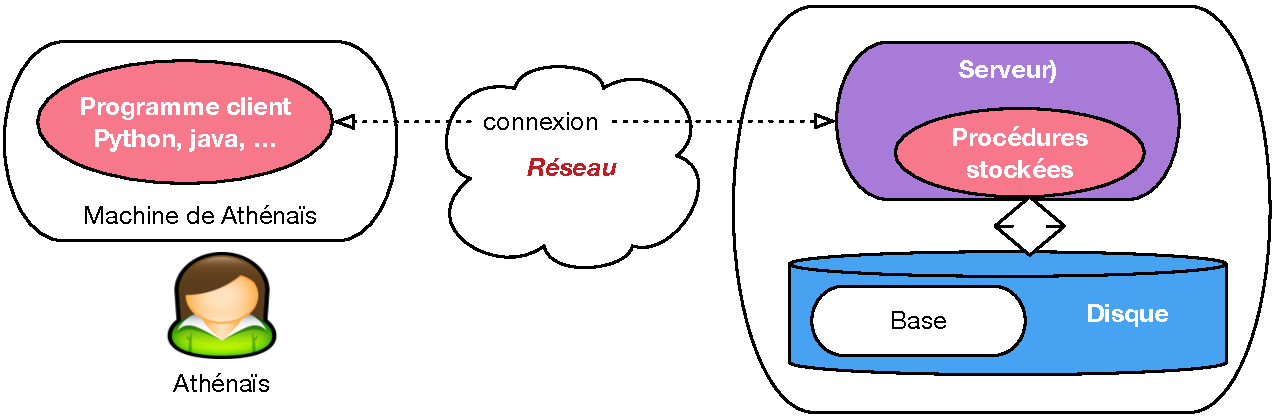
\includegraphics[width=10cm]{../figures-sql/architectures-prog}

\vfill
\begin{blocgauche}
Second cas (à droite)\,:  requêtes SQL  intégrées au \alert{serveur} (procédures stockées)
moins d'échanges réseaux, plus de sécurité.
\end{blocgauche}
\end{frame}


\begin{frame}[fragile]{Premier exemple, mode interactif (PL/SQL)}

\begin{footnotesize}
\begin{minted}{sql}
    DECLARE
      -- Quelques variables
      v_nbFilms   INTEGER;
      v_nbArtistes INTEGER;

    BEGIN
      -- Compte le nombre de films
      SELECT COUNT(*) INTO v_nbFilms FROM Film;
      -- Compte le nombre d'artistes
      SELECT COUNT(*) INTO v_nbArtistes FROM Artiste;

      -- Affichage des résultats
      DBMS_OUTPUT.PUT_LINE ('Nombre de films: ' || v_nbFilms);
      DBMS_OUTPUT.PUT_LINE ('Nombre d''artistes: ' || v_nbArtistes);
    END;
\end{minted}
\end{footnotesize}

\vfill 

\alert{Notez}\,: les variables, la clause \sqlkw{into}.

\end{frame}

\begin{frame}[fragile]{Procédure stockée}

\begin{footnotesize}
\begin{minted}{sql}
    CREATE OR REPLACE PROCEDURE InsereGenre (p_genre VARCHAR) AS 
      v_genre_majuscules VARCHAR(20);
      v_count INTEGER;
    BEGIN
      -- On met le paramètre en majuscules
      v_genre_majuscules := UPPER(p_genre);

      -- On vérifie que le genre n'existe pas 
      SELECT COUNT(*) INTO v_count 
      FROM Genre WHERE code = v_genre_majuscules;
      
      -- Si on n'a rien trouvé: on insère
      IF (v_count = 0) THEN
       INSERT INTO Genre (code) VALUES (v_genre_majuscules);
      END IF;
     END;
\end{minted}
\end{footnotesize}

\vfill 

\alert{Notez}\,: le test.

\end{frame}


\begin{frame}[fragile]{Second exemple, fonction et itérateur}

\begin{footnotesize}
\begin{minted}{sql}
    CREATE OR REPLACE FUNCTION MesActeurs(v_idFilm INTEGER) 
         RETURN VARCHAR IS
      resultat VARCHAR(255);
    BEGIN
      -- Boucle prenant tous les acteurs du films 
      FOR art IN 
        (SELECT Artiste.* FROM Role, Artiste  
        WHERE idFilm = v_idFilm  AND idActeur=idArtiste)
      LOOP
        IF (resultat IS NOT NULL) THEN
          resultat := resultat || ', ' || art.prenom || ' ' || art.nom;
        ELSE   
          resultat := art.prenom || ' ' || art.nom;
       END IF;
      END LOOP;
     return resultat;
    END;
\end{minted}
\end{footnotesize}

\vfill
\alert{Notez}\,: le type automatique de \texttt{art}, la boucle

\end{frame}

\begin{frame}[fragile]{Utilisation}

\begin{redbullet}
  \item En interactif
  \begin{minted}{sql}
     SQL> start StatsFilms.sql
  \end{minted}

 \item Avec l'ordre \texttt{execute}, placé dans un autre langage (C, Java, PHP)
 
   \begin{minted}{sql}
     execute insereGenre('Policier')
  \end{minted}
 
 \item Dans une requête SQL
   \begin{minted}{sql}
      SELECT titre, MesActeurs(idFilm)  
      FROM Film WHERE idFilm=5;

TITRE        MESACTEURS(IDFILM)
------------ -----------------------------
Volte/Face   John Travolta, Nicolas Cage
  \end{minted}
 
\end{redbullet}

\end{frame}


\begin{frame}[fragile]{Dérivation de types depuis le schéma}

Deux exemples pour illustrer.

\vfill

\begin{redbullet}

  \item \texttt{Film.titre\%TYPE} est le titre de l'attribut
     \texttt{titre} de la table \texttt{Film};

  \item \texttt{Artiste\%ROWTYPE} est  un type \texttt{RECORD} 
      correspondant aux attributs de la table \texttt{Artiste}.
\end{redbullet}

\vfill

Le même principe pour les \alert{requêtes SQL} définies dans le cadre des curseurs (à suivre).

\vfill

\alert{Beaucoup plus difficile avec un langage de programmation externe.}

\end{frame}

%%%%%%%%%%%%%
\begin{frame}{À retenir}


Principales difficultés SQL/programmation\,:
\alert{typage} et \alert{conversion}

\vfill

\alert{Typage et conversion des nuplets}

\vfill

\begin{redbullet}
   \item Définir des variables du langage (Python, Java) correspondant aux types
       SQL
   \item Convertir le résultat d'une requête en variables du langage
\end{redbullet}

\vfill

\alert{Typage et conversion des tables}

\vfill

\begin{blocgauche}
Ce sont des \alert{ensembles} (ou séquences si \sqlkw{order by}), on doit les parcourir avec des \alert{boucles}.
\end{blocgauche}
\end{frame}




